\que{Соотношения на поверхностях сильных разрывов в материальном описании.}


Пусть поверхность разрыва $S(t)$ является когерентной, рассмотрим ее образ в $\mathring{\mathcal{K}}$ - поверхность разрыва $\mathring{S}$ и точку $\mathcal{M}\in\mathring{S}$. Построим специальную область $\mathring{V}_h$, называемую \textit{окрестностью поверхности разрыва} и содержащую точку $\mathcal{M}$ (Рис. \ref{risun}). 

% TODO: \usepackage{graphicx} required

\begin{figure}[h!]
	\centering
	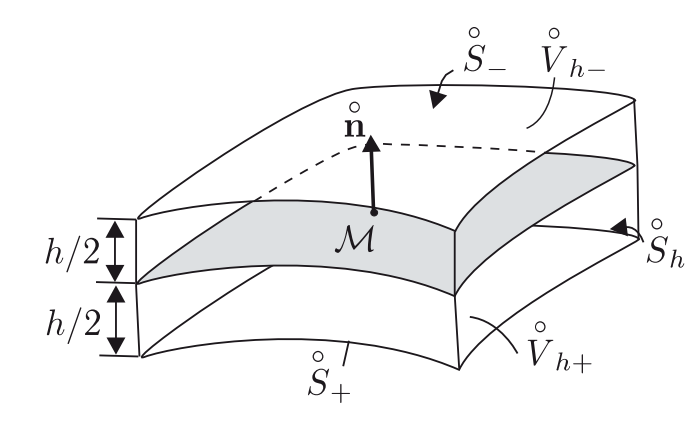
\includegraphics[width=0.7\linewidth]{semester8/img/screenshot001}
	\caption{Область для вывода условий на поверхности разрыва}
	\label{risun}
\end{figure}

Для построения области $\mathring{V}_h$	выберем часть $\mathring{\Sigma}_h$ поверхности $\mathring{S}$, так что $\mathcal{M}\in\mathring{\Sigma}_h$, и введем криволинейные координаты $X^i$ таким образом, что линии $X^1,X^2$ принадлежат поверхности $\mathring{S}$, а линии $X^3$ направлены по нормали к $\mathring{S}$. Область $\mathring{V}_h$ ограничена поверхностью $\partial\mathring{V}_h$, состоящей из боковых поверхностей $\mathring{\Sigma}_{h\pm}$ (их уравнения $X^3=\pm h/2$), торцевых поверхностей $\mathring{\tilde{\Sigma}}_{h\pm}$ (их уравнения $0 < X^3 < h/2$ и $-h/2 < X^3 < 0$, а $X^I,~I=1,2,$ удовлетворяют уравнению контура $\mathring{\mathcal{L}}_\Sigma$, ограничивающую поверхность $\mathring{\Sigma}_h:~X^I=X^I_\Sigma(s),~~0\le s\le s_0$).

Воспользуемся интегральной формой законов сохранения, которые справедливы для произвольного конечного объема, в том числе и для $\mathring{V}_h$:
\begin{equation}\label{eq118}
\frac{\partial}{\partial t}\int_{\mathring{V}_h}\mathring{\rho}\mathring{A}_\alpha d\mathring{V}=\int_{\mathring{V}_h}\mathring{\rho}C_\alpha d\mathring{V}+\int_{\partial\mathring{V}_h}\mathring{\mathbf{n}}\cdot\mathring{B}_\alpha d\mathring{\Sigma}.
\end{equation}
Уравнения сохранения (\ref{eq118}) с учетом теоремы (\ref{eq116}) и условий (\ref{eq17}), (\ref{eq18}) для функций $C_\alpha$ можно записать следующим образом:
\begin{equation}\label{eq119}
\int_{\mathring{V}_{h}}\mathring{\rho} \frac{\partial \mathring{A}_{\alpha}}{\partial t}d\mathring{V}-\int_{\mathring{\Sigma}_{h}}[\mathring{\rho}\mathring{A}_{\alpha}]\mathring{D}d\mathring{\Sigma}-\int_{\partial\mathring{V}_{h}}\mathring{\mathbf{n}}\cdot\mathring{B}_{\alpha}d\mathring{\Sigma}-\int_{\mathring{V}_{h}}\mathring{\rho}\tilde{C}_{\alpha}d\mathring{V}-\int_{\mathring{\Sigma}_{h}}\mathring{C}_{\alpha\Sigma}d\mathring{\Sigma}=0
\end{equation}

Воспользуемся тем, что область $\mathring{V}_h$ выбрана специальным образом, и можно рассмотреть однопараметрическое семейство таких областей, нумеруя их по параметру $h \in (0, h_0)$. Тогда, принимая во внимание, что, согласно аксиоме \ref{ax17}, функции $\mathring{\rho}(\partial \mathring{A}_\alpha/\partial t)$, $\mathring{\mathbf{n}}\cdot\mathring{B}_\alpha$ и $\mathring{C}_\alpha$ являются непрерывными в областях $\mathring{V}_{h\pm}$ и могут иметь только конечный разрыв на $\mathring{\Sigma}_h$, а функции $[\mathring{\rho}\mathring{A}_\alpha]\mathring{D}$ и $\mathring{C}_{\alpha\Sigma}$ - непрерывны на $\mathring{\Sigma}_h$, можно перейти к пределу $h\to0$ (говорят "стянуть область $\mathring{V}_h$ к точке"). В предельном переходе имеют место следующие соотношения:
\begin{equation}\label{eq120}
\begin{aligned}
	&\lim_{ h \to 0} \frac{1}{|\mathring{\Sigma}_{h}|}\int_{\mathring{V}_{h}}\mathring{\rho}\frac{\partial \mathring{A}_{\alpha}}{\partial t}d\mathring{V}=0,
	\\
	&\lim_{ h \to 0 }  \frac{1}{|\mathring{\Sigma}_{h}|}\int_{\partial\mathring{V}_{h}}\mathbf{\mathring{n}}\cdot \mathring{B}_{\alpha}d\mathring{\Sigma}=\mathbf{\mathring{n}}_{+}\cdot\mathring{B}_{\alpha+}+\mathbf{\mathring{n}}_{-}\cdot\mathring{B}_{\alpha-}=\mathbf{\mathring{n}}\cdot(\mathring{B}_{\alpha+}+\mathring{B}_{\alpha-})=\mathbf{\mathring{n}}\cdot[\mathring{B}_{\alpha}],
	\\
	&\lim_{ h \to 0} \frac{1}{|\mathring{\Sigma}_{h}|}\int_{\mathring{\Sigma}_{h}}[\mathring{\rho}\mathring{A}_{\alpha}]\mathring{D}d\mathring{\Sigma}=[\mathring{\rho}\mathring{A}_{\alpha}]\mathring{D},\\
	&\lim_{ h \to 0} \frac{1}{|\mathring{\Sigma}_{h}|}\int_{\mathring{V}_{h}}\mathring{\rho}\tilde{C}_{\alpha}d\mathring{V}=0,~~~\lim_{ h \to 0} \frac{1}{|\mathring{\Sigma}_{h}|}\int_{\mathring{\Sigma}_{h}}\mathring{C}_{\alpha\Sigma}d\mathring{\Sigma}=\mathring{C}_{\alpha\Sigma}
\end{aligned}
\end{equation}

Поделив теперь каждое слагаемое в (\ref{eq119}) на $|\mathring{\Sigma}_h|$ и переходя к пределу $h\to 0$, с помощью формул (\ref{eq120}) приходим к следующей теореме.
\begin{theorem}
	Для системы функций $\mathring{\rho},\mathring{A}_{\alpha}, \mathring{B}_\alpha$ и $C_\alpha$:
	\begin{itemize}
		\item определенной в области $\mathring{V}$ с когерентной поверхность разрыва $\mathring{S}$,
		\item удовлетворяющей аксиоме \ref{ax17},
		\item удовлетворяющей интегральным законам сохранения,
	\end{itemize}
	имеют место следующие соотношения на поверхности разрыва $\mathring{S}(t)$:
	\begin{equation}\label{eq125}
		-[\mathring{\rho}\mathring{A}_\alpha]\mathring{D}=\mathring{\mathbf{n}}\cdot[\mathring{B}_\alpha]+\mathring{C}_{\alpha\Sigma},~~~\alpha=1,\dots,6
	\end{equation}
\end{theorem}